\chapter{The Mu2e Tracker}\label{chaptertrk}

\textit{The following section will focus on the Mu2e Tracker. 
This chapter will give further information about the straw tube Tracker panel, 
including its detection mechanism, the mechanical design and the front end electronics FEE.
As previously pointed out, the Mu2e Tracker is made up of 216 identical panels. 
Each panel is a mechanical and electrical standalone module. Each panel has 96 drift 
tubes used as fundamental detecting components. I will start by discussing the 
theoretical characteristics of drift tubes. Most of the discussion is based on \cite{kola} and XXX.}
\section{Drift Tubes}
Gas detectors are capable of measuring charged particle coordinates. 
They provide great spatial resolution and detection efficiency at a low cost, Ref. \cite{kola}. 
There are many different gas ionizazion detectors, one of these is the drift tube.
The basic configuration of a drift tube is shown in Figure \ref{fig:drifttube}.
The cylindrical conducting tube, the cathode, is grounded.
A hollow cylindrical conducting tube is grounded and serves as the cathode.
The tube is filled with a combination of noble gas, often Argon, and quench gas. 
A thin sensing wire is suspended along the cylindrical cathode axis. 
The wire, called anode, receives a high voltage. Long and thin drift tubes, known as $straw$ $tubes$, have a similar form.
\begin{figure}[!h]
    \centering
    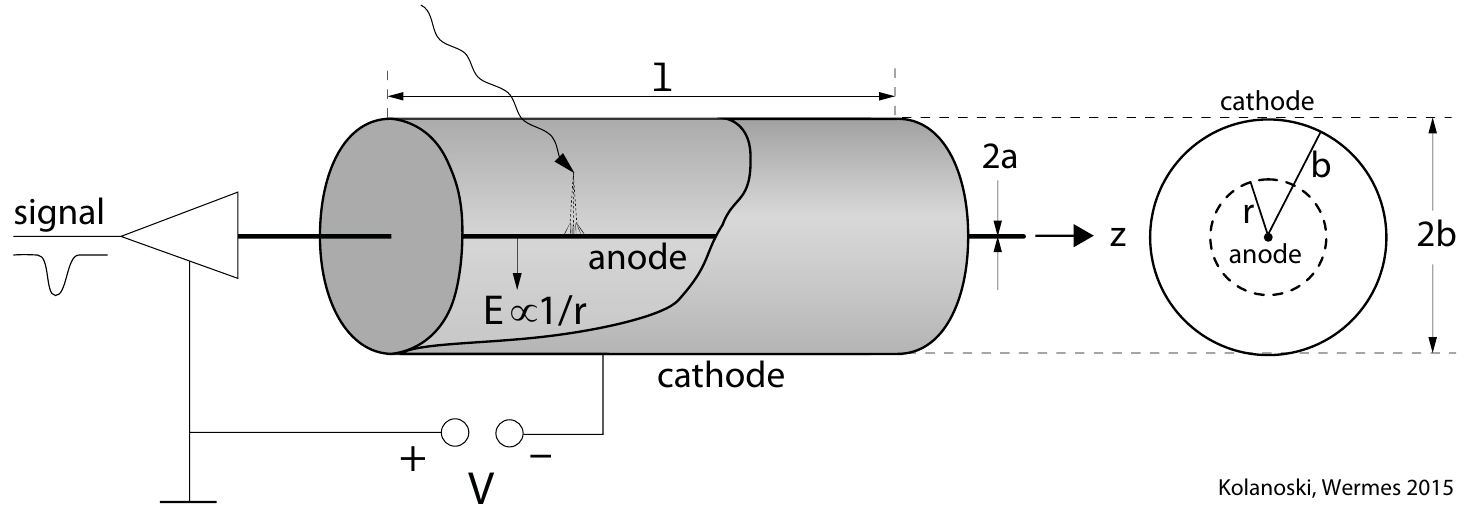
\includegraphics[width =0.8\textwidth]{figures/png/Screenshot_20240324_232621.png}
    \caption{Schematics of a drift tube, Ref. \cite{kola}.}
    \label{fig:drifttube}
    \end{figure}
Assuming an anode radius $a$, a cathode radius $b$ and using Gauss theorem, the electric field is:
\begin{equation}
    E(r)=\frac{1}{r}\frac{\lambda}{2\pi \epsilon}=\frac{1}{r}\frac{V}{ln(b/a)} \qquad (a<r<b)
\end{equation}
Where $\lambda$ is linear charge density on the wire and $\epsilon$ is the dielectric constant of the gas.
Thinner wires are typically preferred in drift tubes. A greater electric field near the wire increases the amplification factor 
of the drift tube at the same voltage. Additionally, smaller wires improve spatial resolution, Ref. \cite{kola}. 
\subsection{Gas Ionization}
\subsection{Drift of Ions and Electrons}
\subsection{Avalanche Multiplication}
\subsubsection{Avalanche Gain}
\subsubsection{Quench Gas}
\subsubsection{Operation Modes of Gaseous Ionization Detectors}
\subsection{Signal Creation and Propagation}
\subsection{Example Detector Responses}
\subsubsection{Minimum Ionizing Particles}
\subsubsection{High Energy Particles}
\section{Tracker panels}
The Mu2e Tracker's straw tube arrays use the same detection principles as the gaseous ionisation detectors, Ref. \cite{kola}, 
but it has a significant different design and manufacturing improvements to meet the experiment precise requirements.
\begin{figure}[!h]
    \centering
    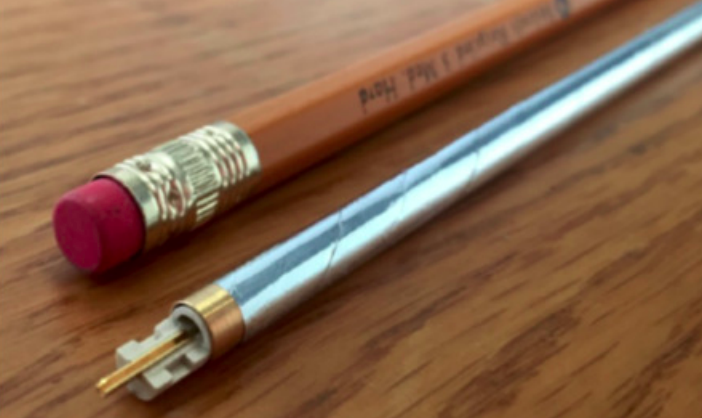
\includegraphics[width =0.5\textwidth]{figures/png/Screenshot_20240327_000000.png}
    \caption{A picture of the Mu2e straw tube
    compared to a pencil, Ref. \cite{trk}.}
    \label{fig:trkpencil}
    \end{figure}
    \begin{figure}[!h]
        \centering
        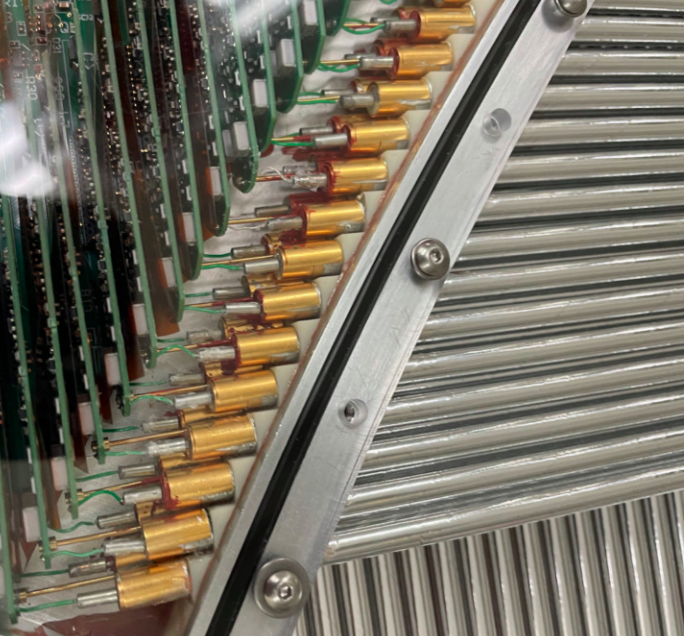
\includegraphics[width =0.5\textwidth]{figures/png/Screenshot_20240327_000131.png}
        \caption{The fully assembled tracker panel with its straws, Ref. \cite{trk}.}
        \label{fig:strawtubes}
        \end{figure}
The straw tubes used in the Mu2e Tracker \ref{fig:trkpencil} are 5 mm in diameter and 0.33 - 1.17 m in length, 
Ref. \cite{bartoszek2015mu2e}. The straws are wound with two layers of 6 $\mu$m-thick metallized Mylar and a 3 
$\mu$m layer of glue in between. The straw wall is 15 $\mu$m thick: this helps to minimize the amout of materials 
in the Tracker, lowering the total energy loss from the observed electrons. Furthermore, it minimises the likelihood 
of significant deflections in electron trajectories, facilitating track reconstruction. As a result, the experiment 
will have a very good momentum resolution. The straw tube anodes are composed of gold-plated tungsten wires 
with a diameter of 25 $\mu$m. The straws and anode wires are tensioned and work-hardened to avoid sagging.
\begin{figure}[!h]
    \centering
    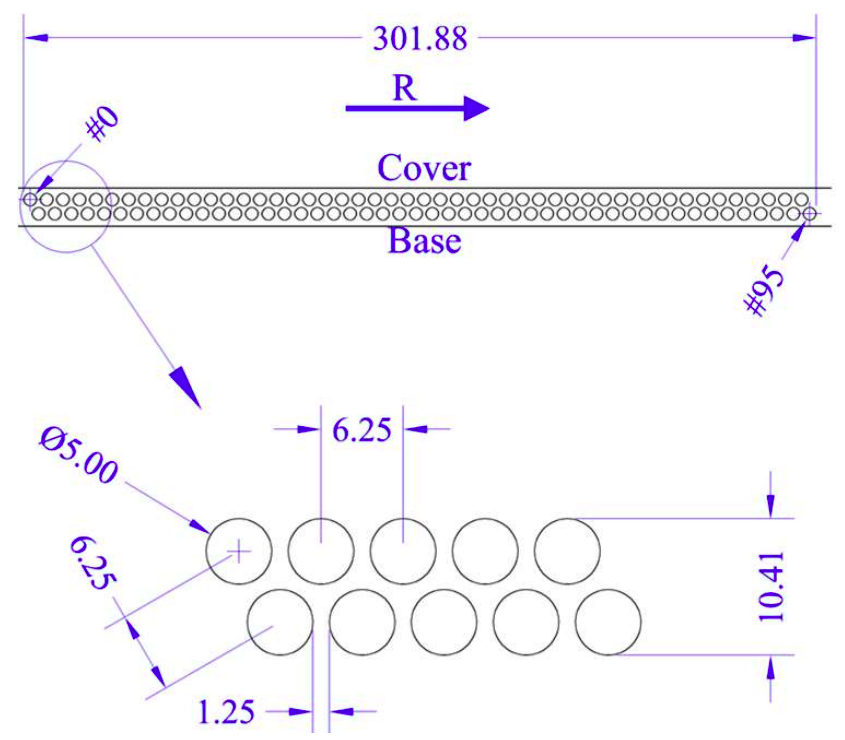
\includegraphics[width =0.6\textwidth]{figures/png/Screenshot_20240326_234405.png}
    \caption{Straw arrangement in a tracker panel, Ref. \cite{trk}.}
    \label{fig:trktubes}
    \end{figure}
To create a perfect electric field with adequate spatial resolutions, the anode wires are oriented 
to the panels with a precision of at least 25 $mu$m in the radial direction and 50 $mu$m in the 
perpendicular direction. All panels are x-ray scanned to accurately measure and document the wire 
locations of straw tube channels for eventual reconstruction. Figure \ref{fig:trkpencil} shows the 
termination mechanism that holds the wire in place.
To increase mechanical strength, a brass tube is joined to either end of the straw using silver epoxied, Ref. \cite{bartoszek2015mu2e}. 
To ensure electrical isolation, a Kapton sleeve is put within the brass tube. An injection-molded plastic insert is then connected 
inside the sleeve. The insert contains a semicylindrical duct that allows gas to enter and exit the straw tube. The insert 
has a groove along its axis and a U-shaped brass anode pin inserted at the end. To avoid slippage, the anode wire is 
epoxied into the groove and soldered to the anode pin.
A T-shaped pin protector protects the anode pin from breaking by covering the groove in the plastic insert. 
The pin protector is epoxied to the insert, with an extra brass ring connecting them. A ground clip 
is silver-epoxied to two adjacent straws on the brass tubes and rings, providing a shared ground connection 
for the straws. 
Signals are sent to a common pre-amplifier (preamp) board via the anode pin pair and grounding clip. 
The FEE will be introduced later. Figure \ref{fig:strawtubes} shows completely built straws in a Tracker panel. 
Each panel has 96 straw tubes organised in two staggered layers for improved tracking. Figure \ref{fig:trktubes} 
show the detailed spatial arrangement of the straws, Ref. \cite{trk}. Channels are numbered from 0 (longest) 
to 95 (shortest), starting with the radially innermost straw.
Straws are spaced by 1.25 mm and can expand under gas pressure, Ref. \cite{bartoszek2015mu2e}.
The Mu2e Tracker panels employ a gas flow of 80\%:20\% Ar:CO$_2$. 
The vacuum environment within the Detector Solenoid reduces the impact of electron scattering on trajectories. 
However, the Tracker panels, particularly the straws, must endure pressure differences. Under normal temperature 
and pressure, each panel must have an average leak rate of 0.014 cm$^3$/min. The nominal operating voltage of 
the straw tube channels is 1450 V. An earlier investigation on a prototype of the Tracker showed the straw tube 
gain as 1.25 $\times$ 10$^4$ at 1250 V and 7 $\times$ 10$^4$ at 1425 V. According to Diethorn's calculation, Equation \ref{XXX}, 
the gas gain at 1450 V is around 1 $\times$ 10$^5$.

\section{Tracker Front-End Electronics}
Before being accessible to the Mu2e Data Acquisition (DAQ) system, the analog signals 
from the Tracker straw tube channels need amplification, digitization and packaging. 
The Tracker front-end electronics (FEEs) are designed to achieve these goals. The FEEs 
consist of multiple Printed Circuit Boards (PCBs) as shown in Figure \ref{fig:trackerfee} \cite{vadimmu2e}.
All PCBs are situated in the outer section of the panel. Pulse timing is measured at the 
end of each straw, in order to be able to measure electron position on the wire. A measure 
of $dE/dx$ is provided, so pattern recognition can be possible, Ref. \cite{bartoszek2015mu2e}. For this purpose each straw has:
\begin{itemize}
    \item two preamp channels, one for each end;
    \item two TDC channels, one for each end;
    \item one ADC channel, measuring sum of both ends;
    \item one High Voltage feed.
\end{itemize}
There are 46,080 preamps and TDCs and 23,040 ADC channels. There are two sides of the panel, one called HV side and one called CAL side. 
\begin{figure}[!h]
\centering
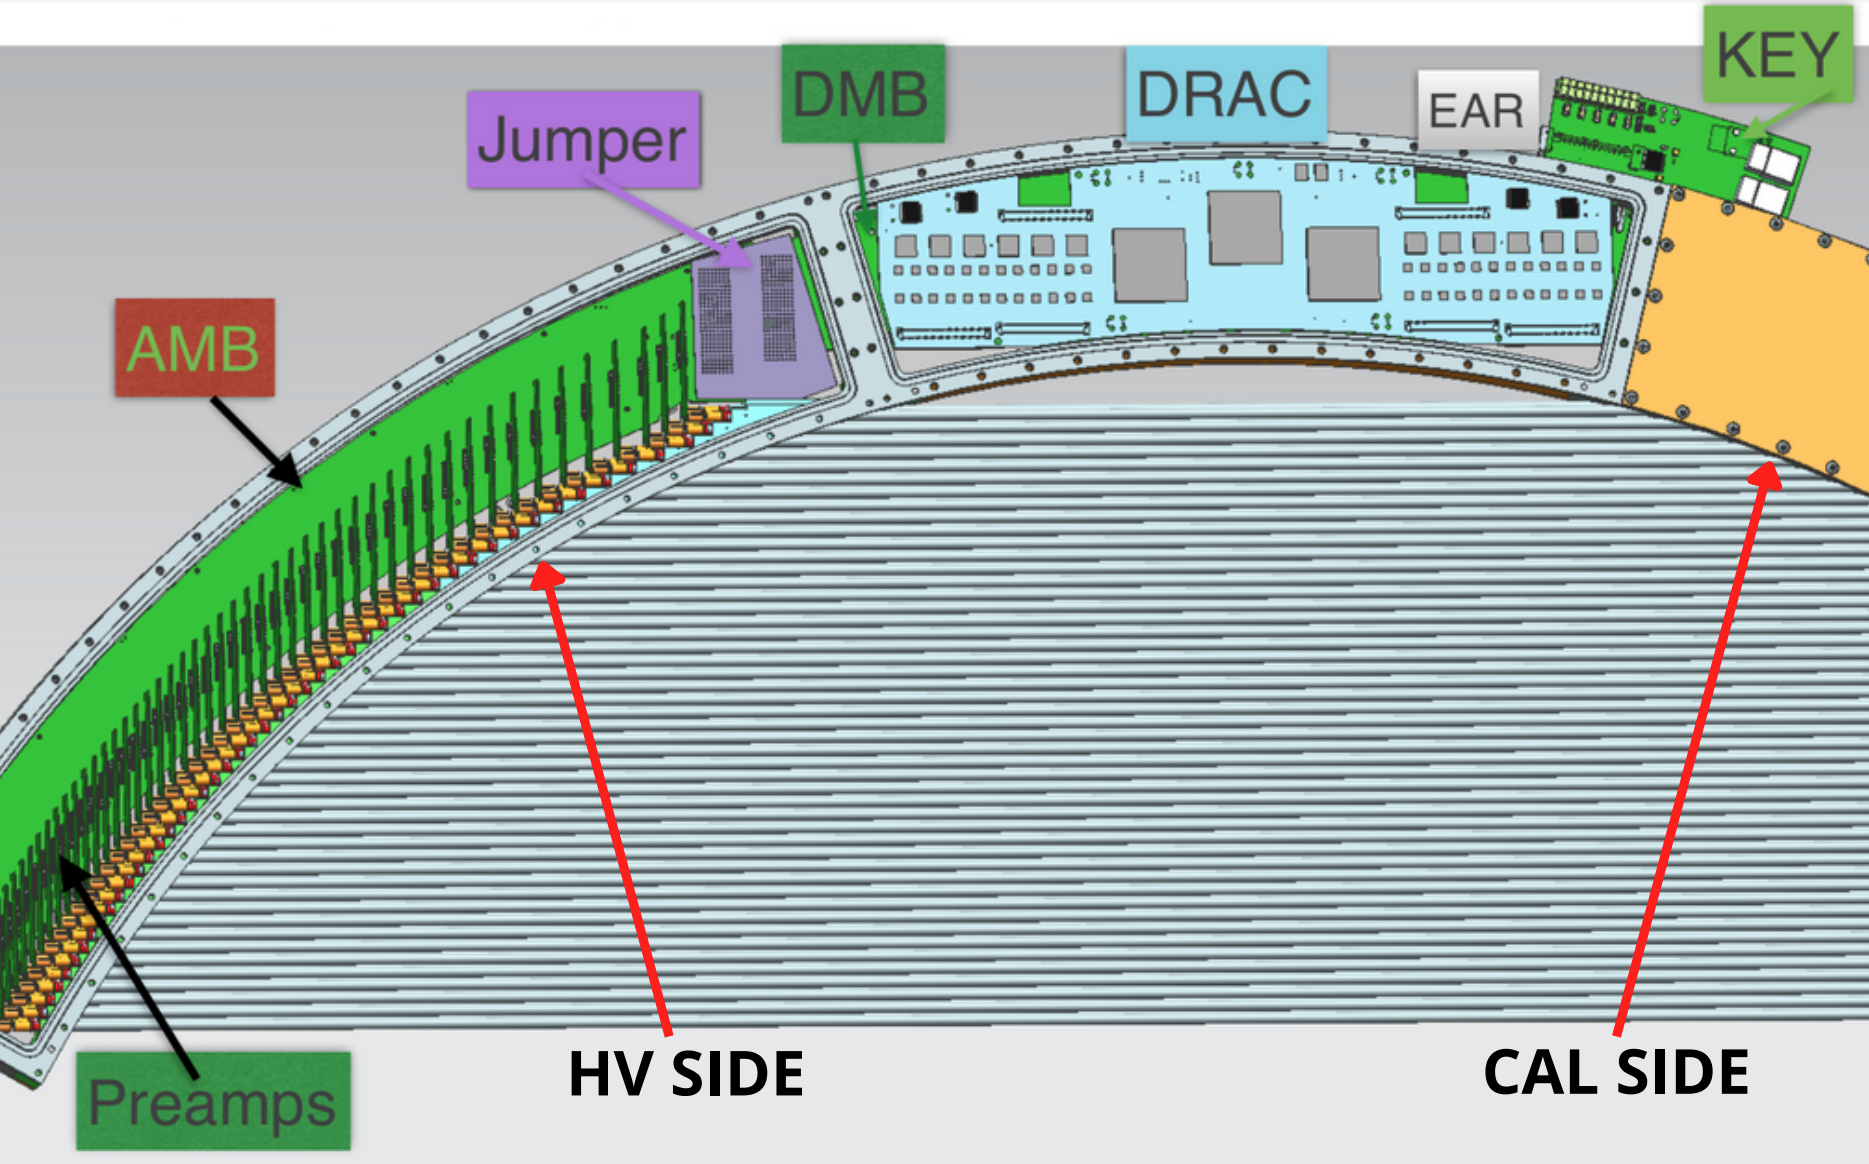
\includegraphics[width =0.8\textwidth]{figures/png/Screenshot_20240131_111836.png}
\caption{An overview of the Tracker front-end electronics (FEE) 
\cite{vadimmu2e}. The preamps and the Analog Motherboard (AMB) 
on the other side of the straws are not shown in the figure.}
\label{fig:trackerfee}
\end{figure}
On either side, there are an Analog Mother Board (AMB) and a Jumper board, 
which task consist of directing signals from the preamps towards the Digital 
Motherboard (DMB) positioned at the center, then to the Digitizer Readout and 
Assembler Controller (DRAC) (mounted on top of the DMB) to be processed and 
temporarily stored. Both the AMBs and the DMB handle low voltage distribution 
and the HV side of the AMB distributes high voltage to the straw anode wires, 
reason why it is called this way. On the AMBs and the DMB there are sensors, 
monitoring environmental variables such as temperature, pressure and humidity. 
The low voltage power supply is fed into the panel through the KEY. The KEY 
contains an optical fiber link and a JTAG interface for communication. The 
frontends components were chosen to sustain high level of radiation.
\subsection{Pre-Amplifiers}
The pre-amplifiers (preamps) are responsible for the initial readout of 
signals from both ends of the straw tube channels. As previously explained, 
the channels are read out from both ends and two adjacent channels are linked 
to the same preamp. Each tracker panel contains 48 preamps on the HV side, 
while an additional 48 preamps are located on the opposite side, the CAL one. 
Preamps are mounted vertically on the AMBs. Preamps are required to have a 
matching 300 $\Omega$ input impedance with the straw, in order to avoid signal 
reflections. The preamps convert the straw tube current signals into voltage signals. 
Signals are amplified and shaped. The preamps on the CAL and HV sides aren't 
exactly the same. The CAL preamps have circuitry that can inject calibration 
pulses into the channel. This capability enables the channel readout electronics 
to be tested without a high voltage source. The preamps on the HV side distribute 
the high voltage supply to individual straw tubes. 
%The voltage gains of individual channels, different from the gas gain, are set by control signal from the DRAC. A bias voltage, adjustable for each side of a channel, is applied to the signals. 
\subsection{Digitizer Readout and Assembler Controller}
The brain of a tracker panel is called Digitizer Readout and Assembler Controller (DRAC). 
The DRAC is responsible for digitizing, packaging and temporary storage. It also controls 
panel operations. The schematics of the DRAC board is shown in Figure \ref{fig:drac}. In 
this figure Analog to Digital Converters (ADCs), DDR3 memories and compators are shown. 
The large chips in the centers are the Field-Programmable Gate Arrays (FPGAs). The one 
in the center is the Readout Controller (ROC), which manages communications, monitors 
slow control variables and controls panel operations \ref{ROC}. The left and the right 
ones, which are referred to as the DIGI FPGAs, are responsible for monitoring data output, 
buffering data and assembling data packages. Each of them refers to 48 straw channels. 
\begin{figure}[!h]
\centering
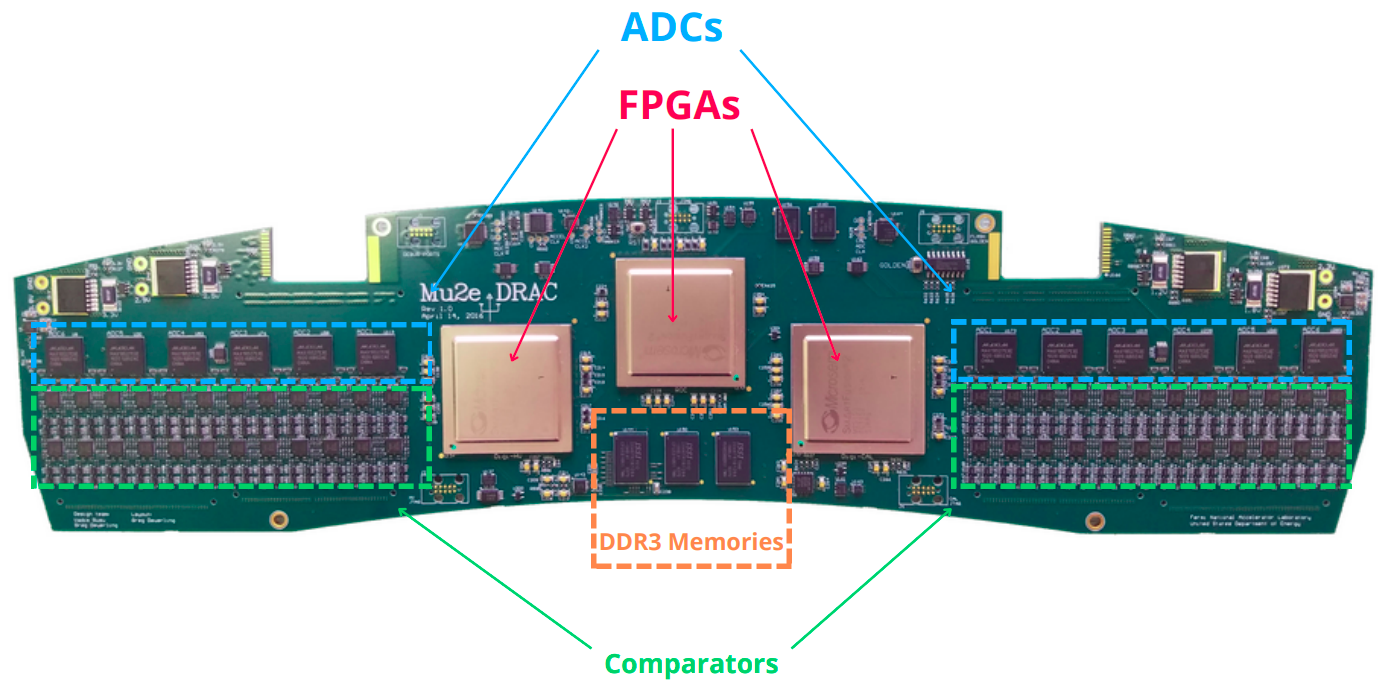
\includegraphics[width =\textwidth]{figures/png/Screenshot_20240204_115052.png}
\caption{Digitizer Readout and Assembler Controller (DRAC) board schematics \cite{drac}. 
The DRAC board is the brain of the tracker panel. In this figure Analog to Digital Converters (ADCs), FPGAs, DDR3 memories and compators are shown.}
\label{fig:drac}
\end{figure}
In figure \ref{fig:flowfee}, signal flow in the Tracker FEEs is reported. At the 
beginning the signal coming from both ends of the straw is routed to the preamps. 
After that, the analog signal is sent through the microstrip transmission line to 
the digitizers. In the DRAC, the two biased signals are fed independently to 
zero-crossing comparators, which produce square pulses when the signals exceed 
their respective thresholds. The squared pulses are sent to Time-to-Digital Converters 
(TDCs, firmware based, 16 bits each) implemented in the DIGI FPGAs, that have the task 
of digitizing the trigger timings, including the arrival time and the time over threshold, 
at a rate of about 62.5 MHz. Besides drift time, TDCs measure time difference across the 
straw to estimate position along the wire and the intrinsic time resolution of TDC is about 
25 ps, adding comparator jitter, noise and other external effects the final resolution is 
$\sim$ 70 ps for time division. Furthermore, an integrator adds voltage signals coming 
from the two straw ends. In data collection, a hit occurs when both ends of a straw channel 
are simultaneously activated. The total is digitized by a 12-bit (10-bit ENOB) ADC at 50 MHz 
and then sent to the DIGI FPGA. The DIGI FPGA creates a data packet for each hit based on 
TDC and ADC information. This suppresses false triggers caused by random electrical noise. 
The Digitizer receives signals from both ends of four straws and multiplexes them into one 
output buffer before sending a packet of data to the ROC. Signals are sent to the ROC at 
200 MHz. The data packets are then briefly stored in DDR3 memory for further use by the 
DAQ system. It is important to save also the voltage signal, since the pulse height 
information can help us to reject proton background, a significant source of noise 
or to distinguish muons from electrons. The proton signal will appear as a saturated flag, 
since the proton $dE/dx$ is $\times$50 the electron one.
\begin{figure}[!h]
\centering
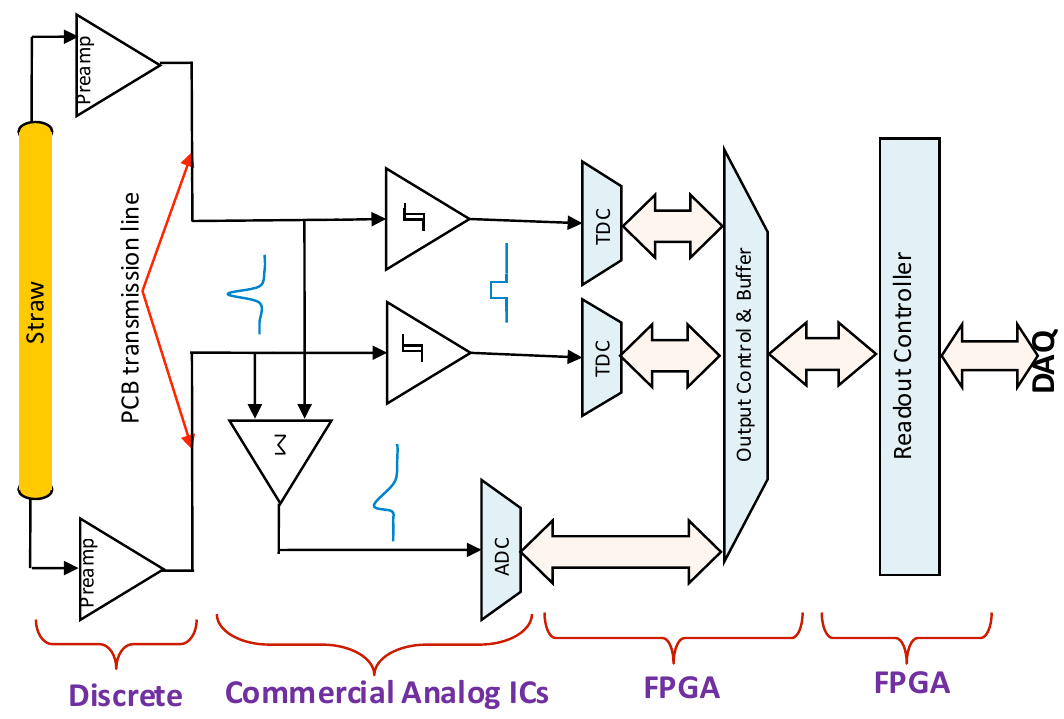
\includegraphics[width =0.8\textwidth]{figures/png/Screenshot_20240203_135048.png}
\caption{Signal flow through front end electronics \cite{bartoszek2015mu2e}.}
\label{fig:flowfee}
\end{figure}

\subsection{Read-Out Controller}\label{ROC} 
The main job of the ROCs (one per panel, 216 in total) 
is to collect data from the digitizer boards, buffer data and 
send them to DAQ. They are based on an FPGA architecture. They 
continuously streams out the zero-suppressed data collected between 
two proton pulses from the detectors, in this case the tracker, to 
the DTCs (Data Transfer Controller)\cite{GIOIOSA2023167732}. The buffer 
stage is fundamental, since during the beam inter-spill time (836 ms 
out of each 1333 ms), we want us to be able to take data from cosmic 
rays, even if the rate will be very low. For this purpose, the ROCs 
include external DRAM. The communication is flexible, thanks to the 
programmable nature of digitizer, ROC and DAQ. 

XXXX immagine 
